\documentclass[UTF8]{ctexart}
\author{王秋里} 
\title{机器学习算法之深度神经网络RNN\\从自然语言处理到软件仓库挖掘} 
\usepackage{geometry}
\geometry{left=2.0cm, right=2.0cm, top=2.5cm,bottom=2.5cm}
\usepackage{indentfirst}
\usepackage{graphicx}
\setlength{\parindent}{8em}

\begin{document}  
	\maketitle   
	\section{自然语言处理}      
			\paragraph{}
			图灵在1950年提出:如果一台机器能够与人类展开对话(通过电传设备)而不能被辨别出其机器身份,那么称这台机器具有智能。这其中就涉及到人与机器通过自然语言交流。所以,通常来说,人们把1950年看成是NPL发展的元年。自然语言处理发展的第一阶段是1950年到1970年。在那段时间内,人们普遍认为,如果要让机器完成翻译或者语音识别等只有人来才能做的事情,第一,首先要让计算机理解自然语言;第二,要做到第一点,就要让计算机拥有类似于我们人类这样的智能。但是当时人们并没有意识到这是一个错误的方向。通常我们学习一门语言的时候,我们会通过学习它的语法规则,词性和构词法来了解这一门语言。这一个方法在我们人类的学习生活中被证明了是有效的。而且,语法在计算机中较为容易表达,所以当时人们坚信可以让计算机通过语法来进行机器翻译。但是,其实这种方法是有很大缺陷的。我们先来看一个例子:徐志摩喜欢林徽因,它的语法树如图1所示。
\begin{figure}
\centering
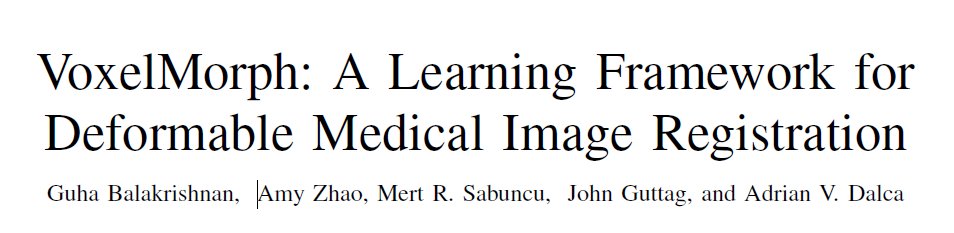
\includegraphics[totalheight=5cm]{1.png}
\caption{语法树}
\label{fig:test}
\end{figure}
			这是一个很短的句子,但是他的语法树却没有我们想像中的那么小巧。当然这样的一句话还是可以在计算机中通过语法树来表达。但是,如果是很长的一句话呢?再来看一个例子.Pen is in the box,这句话对我们来说很容易理解,但是倒过来:Box is in the pen,这句话对我们来说就很难理解了,因为盒子怎么会在笔里面呢?但是对于英国人来说这句话就很容易理解,因为pen还有围栏的意思。英国人结合前后语境,很容易就可以理解这句话。这个例子说明,有的时候翻译是需要结合前后语境的,但是语法树很难处理这样的问题。所以在这个时期,人们虽然花了大量精力去做NLP,但是效果提升不明显。直到20世纪70年代,弗里德里克-贾里尼克提出了用统计的方法来解决自然语言处理的问题,NLP这才进入了新的一页。
			\paragraph{}
			贾里尼克的想法很简单,就是通过统计的方法来判断这个句子存在的可能性。贾里尼克认为,一个句子是否合理,就看它的可能性大小如何。比如一次翻译给出了三个结果,第一个结果出现的概率是10$^{-20}$,第二个结果出现的概率是10$^{-30}$,最后一个结果出现的概率是10$^{-70}$,那么我们就会认为,第一个句子出现的概率最大,那么它翻译正确的概率也就最大。如何来计算一个句子存在的可能性呢?假定S表示一个有意义的句子S = (w$_{1}$, w$_{2}$, w$_{3}$, w$_{4}$, w$_{5}$, w$_{6}$……w$_{n}$),那么ps等于P(w$_{1}$)P(w$_{2}$|w$_{1}$)P(w$_{3}$|w$_{1}$,w${_2}$)……P(w$_{n}$,|w$_{1}$,w$_{2}$,w$_{3}$,…w$_{n-1}$)
但是这样的公式有一个问题,就是句子如果长度很大,那么这个概率计算的公式将会十分复杂,那么这样的统计也会变得成本很大,那么接下来,马尔科夫假设就解决了这个问题。马尔科夫假设大概意思是假设任意一个词wi出现的概率只同它前面的词wi-1有关。这样,这个句子出现的概率就变得较为容易计算。公式可以简化为P(S)=P(w$_{1}$)P(w$_{2}$|w$_{1}$)P(w$_{3}$|w$_{2}$)…P(w$_{n}$|w$_{n-1}$)

			\paragraph{}
			现在,我们手里有了模型,就可以把模型放到计算机里了。接下来我们就要考虑,如何把语言放入计算机进行处理。通常来说,我们要将每一个单词表征为一个d维的向量,我们希望通过填写值得方式,让向量表征词。一句话的每一个单词用向量表示之后,我们就可以用一个共生矩阵来表示这句话。假设一句话为:I love NLP and like dogs。我们可以来观察一下这句话。我们可以发现,love(101000)和like(100001)的向量和I(010110)的向量相连的次数都是1,那么这个我们可以猜测,101000和100001所表示的词和010110的关系是相近的。在对大量的词进行统计之后,我们可以观察到很多这样类似的关系,比如King相对于man的关系,类似于Queen相对于woman。那么通过这样的方法,我们就能够用共生矩阵来获取某一种语言的特征。这个也是以后将机器学习用在NLP的基础。
		\section{RNN与自然语言处理}
			\paragraph{}
			首先我们要问一个问题,既然马尔科夫模型可以进行一些语言的预测,为什么还要用到RNN呢?这是因为马尔科夫模型对过程状态的预测虽然效果不错,但是它不适合用于系统中长期的预测,句子如果很长,那么马尔科夫模型很难把握句子的信息。而且他的学习网络同样也有一些缺陷,比如他们会要求所有的输入都是一次性输入,输入的长度是固定的,而语言本身长度是不定的。由于这一特性,其他网络往往要求输入层要足够长,能够包含绝大部分语句的长度。用RNN则可以很好的解决这个问题,因为RNN没有这些要求,非常适合序列信息的处理。LSTM模型可以很好的解决长期依赖的问题,它可以很好的保留语言中相隔距离较长但是却十分有用的信息。在这里我则要详细看一下另外一个模型GRU,门控制循环单元,如图2所示。
\begin{figure}
\centering
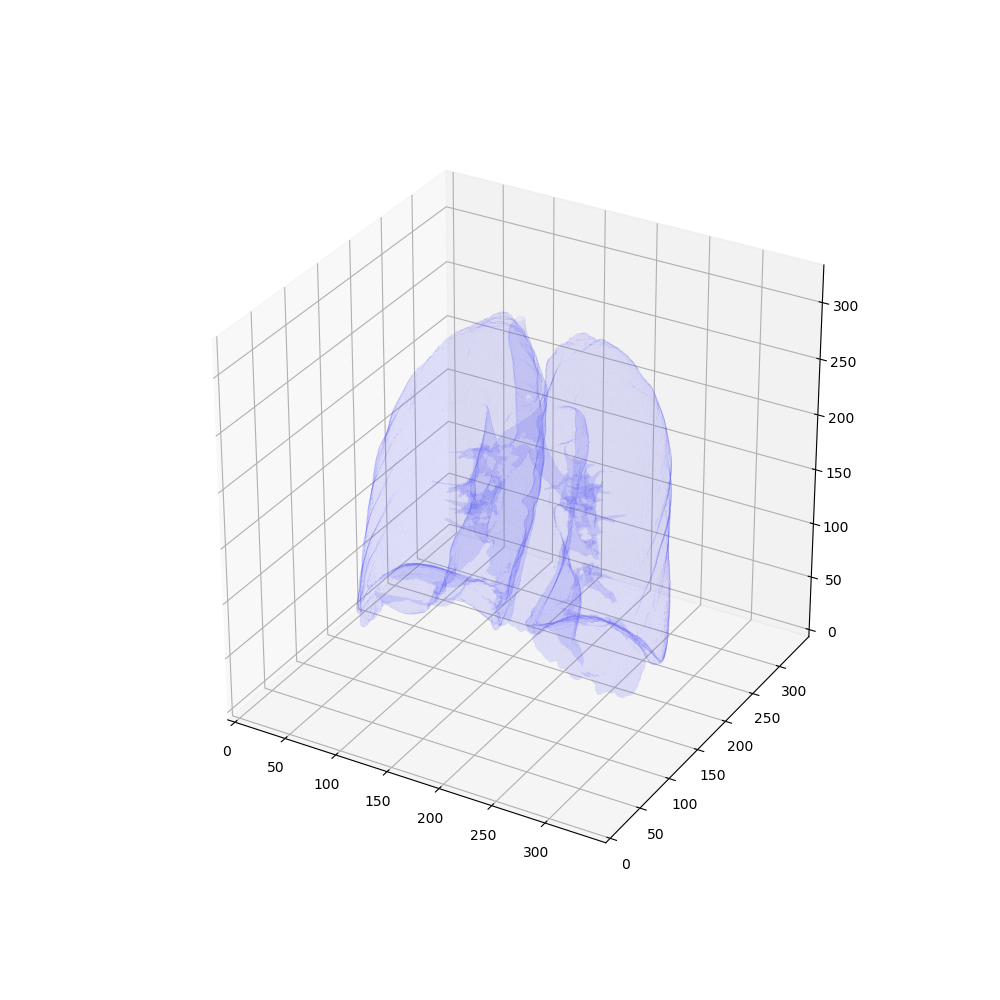
\includegraphics[totalheight=5cm]{2.jpg}
\caption{GRU}
\label{fig:test}
\end{figure}
它和LSTM相比,结构更为简单,少了一个门,但是它的效果却和LSTM不相上下。这样,我们实际的编码可以简化很多。那么这个GRU又有什么特点呢?首先我们看一下,在GRU中,它提供了一个更新门,一个重置门,以及一个记忆存储器。那么他们是通过以下公式进行更新的:
$$z_j=\sigma([W_z x]_j+[U_z h_{<t-1>}]_j) $$
$$r_j=\sigma([W_r x]_j+[U_r h_{<t-1>}]_j) $$
$$h_j^{<t>}=z_j h_j^{<t-1>}+(1-z_j)\widetilde{h_j}^{<t>}$$


$$\sum_{i=1}^n a_i=0$$

我们要注意的是,zj和hj是用的权重是分开的,不一样的。
			\paragraph{}
			update gate控制当前时刻的隐藏层输出h$_{t}$,控制h$_{t}$需要保留多少之前的隐藏层信息, 若z$_{t}$接近1相当于我们之前把之前的隐藏层信息拷贝到当前时刻,可以学习长距离依赖。如果reset gate接近0,那么之前的隐藏层信息就会丢弃,允许模型丢弃一些和未来无关 的信息。一般来说那些具有短距离依赖的单元reset gate比较活跃(如果rtrt为1,而ztzt为0 那么相当于变成了一个标准的RNN,能处理短距离依赖),具有长距离依赖的单元update gate比较活跃。由这样的GRU组成的网络,就可以较好的处理NLP问题。我们这里要看的是RNN Encoder Decoder模型。和最开始的模型不同,这个RNN Encoder Decoder里面的每一个单元,都是GRU。Encoder Decoder模型作用是,将一个可变长度的序列学习映射成一个长度固定的向量,然后再用这个向量去处理一个可变长度的序列翻译的问题。这个模型有两个RNN网络,下面这个RNN隐藏层更新的公式是
$$r_j=\sigma([W_r x]_j+[U_r h_{<t-1>}]_j) $$

上面Decoder隐藏层更新的公式是

我们要注意到的是,上面这个Decoder隐藏层不仅仅收到C的影响,同时还会收到前一次输入y-1的影响。
			\paragraph{}
			这里举一个自然语言翻译的例子。在一篇论文《Learning Phrase Representations using RNN Encoder–Decoder for Statistical Machine Translation》里,作者制作了一个英语翻译到法语的模型。首先他们从一个2G的词语资料里筛选了418M的词语用来建模,从850M的词语资料里筛选了348M用来训练。训练的过程大体如下。。。。我们要注意的是,这里的向量C是等所有的X都输入之后训练得到的。这是它的一个特点,我们在后面会看到另外一种Encoder Decoder模型,它对这个C以及下面的Encoder做了一些改进。
			\paragraph{}
			这就是它的一个翻译结果。左边是他们输入的source,右边则是这个模型得到的次数最多的结果。
			\section{软件仓库挖掘--API Learning}
			\paragraph{}
			这个部分,我们以一篇论文为基础讲起。论文名叫《deep api learning》,作者叫顾小东,现在是香港科技大学在读博士。他主要研究的方向就是deep learning, SE, 以及Code Search方面的一些工作。这篇文章的主要思想就是,通过深度学习,加强对搜索语义的理解,提高API搜索的正确性。
			\paragraph{}
			首先我们要看一下,deep api learning和先前的方法有什么区别。这是stack overflow的界面,我们输入java save string to file,这个时候搜索出来的结果是通过关键字的比对来得到的。我们可以看到,凡是匹配了关键字的地方,搜索结果都会进行显示。这样的关键字搜索有比较明显的缺陷。我们来看下面一张图。这是stack overflow里面的两个问题。这两个问题分别是1.。。2.。。,我们可以看出,这两个标题关键字的匹配程度不高,说明搜索的时候,这两个标题搜索出来的结果应该不一样。但是实际上,这两个问题几乎可以用同样的方法来解决。也就是说,搜问题1的人,就不会搜到问题2的解决方法,尽管说,问题2的答案可以很好的解决问题1。现在我们搜索API基本上还是用的通用的搜索引擎,比如Google,程序员用stack overflow多一些,但是这些搜索引擎都是基于关键字的搜索。关键字搜索的缺陷主要有以下三个:1,2,3.
			\paragraph{}
			为了克服这些缺陷,有些研究人员也做了一些工作。比如在code search领域,McMillan构建了一种模型,他把代码当作网络来看,每一个api或者是函数都是一个网页,利用pagerank算法,对两个“网页”进行分析,A与B的关联度越高,那么调用A的时候,B出现的可能性也就越大,那么通过这个方法,将关联性价高的api关联起来,提高搜索准确度。而Fowkes则是对api使用的模式进行识别。但是他并不知简单的去提取信息。而是对有用的模式进行提取。比如左边这里,一长串的println函数,对于系统来说并不是最重要最有用的api,这种重复无效的api作者会忽略。而右边这个图片里的api对系统来说则重要的多,它实现了系统的某些功能。这些对于系统有价值的api模式才是作者需要提取的。通过这样的方式,可以帮助用户找到他想要的api。但是以上两种方法都没有解决最根本的问题:关键词匹配无法理解用户输入的信息,不能捕获到语义信息。
			\paragraph{}
			我们先看一下顾晓东这个小组做出来的成果。这是他们的页面,上面用户查询的输入框。在我们输入一个问题的时候,这个平台会给出最符合用户需求的API调用顺序,越往上,越接近用户的查询。我们看一下,这张图是其他查询所输出的效果。可以看出来这个查询准确率还是很好的。那么它是怎么实现这个功能的呢?这就要结合我们之前提到的模型RNN Encoder Decoder。这是这个系统模型的一个图片展示,总体来说它是和之前的RNN Encoder Decoder相似的。但是它在某些细节上做了调整,这样可以让整个系统的效果更好。那么它和之前的Encoder Decoder有哪些不同呢?
			\paragraph{}
			首先第一点不同,也是它最直观的特点,就是它的输入输出。之前Encoder Decoder输入输出都是自然语言,而在这里,它的输入是具有自然语言注释标签的api序列,而它的输出是一个api的序列。我们其实很好理解作者为什么会想到用这个模型。因为api的调用顺序其实也是可以当成一种语言来看的。它这里做了一个概念上的置换。它通过以下的方法来提取输入的数据。首先先通过一个转换,将一段程序转换成api的序列,具体我们看一下,这里列出了6种代码的模式,第一个是新建一个类,第二个是调用一个方法,第三个是一个带参数函数的调用。第四个是顺序语句,第五个ifelse,最后一个是while循环。右边是它转换的一个公式。我们可以看到这其实是一个很简单的转换,并且这些转换是一一对应的,基本上可以涵盖绝大部分代码的结构。这个转换的过程就是去分析代码,将代码相应部分变成这个顺序,然后放到它的api序列。这样的话,api序列我们就能得到了。接下来是获取注释信息。这里就对程序的格式要求比较高了。他要求这个Java项目是严格按照Java文档的要求来做的。也就是说,在正规文档的要求中,这样的注释要求第一行用来描述这段代码的作用。在符合要求的Java项目中,他们将提取注释的第一行,当作这段api序列的注释标签。这是一整个代码的样例,按照上述方法来提取信息之后,我们可以得到以下的结果。现在我们需要的数据已经得到了,那么我们怎么来训练呢?
			\paragraph{}	
			我们再来回顾一下模型,之前提到,在这个模型里对传统的Encoder Decoder网络进行了改进。它具体的改进有两点:一个是对于c向量的改进,一个是对于encoder网络的改进。这张图标注出这篇文章用到的Encoder Decoder和传统的Encoder和Decoder的区别。第一个是c向量。之前的EC网络,我们说,要等所有的x都输入结束,才能将c向量拿来训练decoder,但是在这里,针对每一个输出y,都会有一个特定的c向量来处理,也就是说,c向量再也不是固定的了。第二,传统的encoder网络只有一个rnn网络,但是在这里,encoder有两个rnn网络,并且一个是正向网络,一个是负向的。那么这些改动具体是为了解决什么问题的呢?
			\paragraph{}
			我们知道,在之前的ed网络中,解码器仅依赖编码器最后的隐藏状态。c向量必须对源句子所有的内容都进行编码/它必须充分的捕捉含义。然而,我们似乎无法把一个很长的句子所包含的信息编成一个向量,然后解码器仅根据这个向量生成完美的翻译,这种假设是很难成立的。我们假设原文句子长度有50个单词,英文翻译的第一个单词可能与原文的第一个单词高度相关。但是这意味着,编码器必须考虑50步之前的信息,而且那段信息需要以某种形式编入向量中。我们知道,RNN在处理长距离依赖关系的时候容易出问题,理论上,LSTM这类结构能够处理这个问题,但是在实践中,长距离依赖关系依然是个问题。但是研究人员发现,将原文倒序输入编码器会产生显著的效果,但是这种方式并不适合所有语言,因为某些语言句子最后一个词语在英语翻译中对第一个词具有高度的语言性。
			\paragraph{}
			解决这个问题的方法就是attention机制,我们不需要将完整的原文句子编码为固定长度的向量。相反,我们允许编码器在每一步输出的时候参考原文的不同部分。更重要的是,我们让模型根据输入的句子以及已经产生的内容来决定参考哪一部分。因此,在形式非常相近的语种之间,解码器可能会选择顺序的参与生成。每个编码器输出的词语yt取决于所有输入状态权重的一个组合,而不是只有最后一个状态。因此,如果a2、a3的值很大,这意味着解码器生成译文的第三个单词的时候,会更关注原文句子的第二个状态。a求和的结果通常会进行归一化,它是输入状态的一个分布。双向rnn不仅可以捕获x之前的信息,而且可以捕获x之后的信息,这有助于翻译的准确性。
			\paragraph{}
			这是所有attention模型的公式。这些公式看起来十分复杂,但是实际上分解开来都是比较基本的公式。这里hj其实是正向hj和反向hj对应位置的一个组合。那么现在训练的过程也明确了,我们就可以开始训练了。最后展示一下这篇论文里训练的结果。这是对所有训练结果的一个投射,我们可以看到,语义比较相近的句子聚集在了一起。最后是他搜索过程的一个可视化
			\paragraph{}
			那么这个模型的基本信息就是这些。说是来将这篇论文,其实是借这篇论文介绍一下更有效的编码解码模型,希望大家能够有所收获。














\end{document} 